\documentclass{article} 
\usepackage{listings}
\usepackage{graphicx}
\usepackage{subfig}
\usepackage{multirow}

\lstset
{ %Formatting for code in appendix
    language=Python,
    %basicstyle=\footnotesize,
    numbers=left,
    stepnumber=1,
    showstringspaces=true,
    tabsize=4,
    breaklines=true,
    breakatwhitespace=false,
}

\title{AI 534 IA1 Report}
\author{Rishab Balasubramanian}
\date{}

\begin{document}
\maketitle
\textbf{Part1.}a. The smaller learning rates upto $1e-5$ were very slow, and did not convege within $5000$ iterations. The learning rates between $1e-4$ and $0.1$ worked well, with $lr=0.1$ giving the best performance. The other rates aboe $0.1$ immediately caused the loss to diverge. Fig. \ref{fig:normalized} shows the plots for MSE vs Iterations for different learning rates.\\
 
b. The MSE of the Validation Data is reported in \textbf{Part1.pdf}. The best validation is given by the learning rate $0.1$. I think the best learning rate is the one that gives maximum reduction in loss, without divergence. In out case this was $0.1$. At any point however if the loss seems to diverge, we can stop training and continue with a lower learning rate.\\

c. A Learning rate of $0.1$ works best and results in a MSE of $3.757$ on the training data and $4.501$ on validation data. The learned weights are provided in \textbf{Part1.pdf}. Of the given features, $grade$, $sqft\_above$, $age\_since\_renovation$ and $waterfront$ are the top $4$ most important features.\\


\begin{figure}[h]
    \centering
    \subfloat[\centering Learning Rate = 1e-8]{{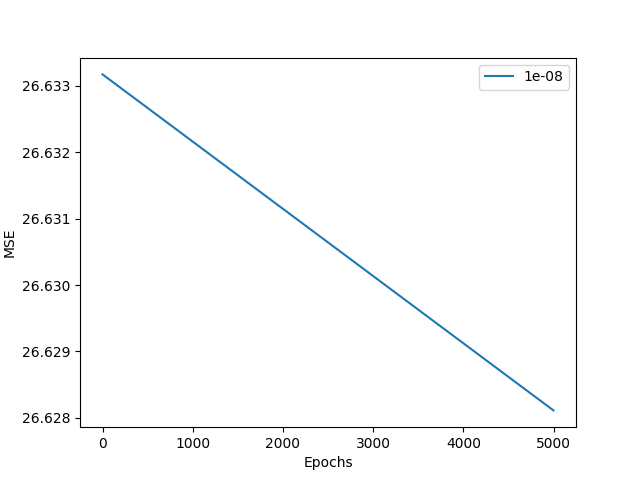
\includegraphics[width=0.32\textwidth, height=4cm]{1e-8} }}
    \subfloat[\centering Learning Rate = 1e-7]{{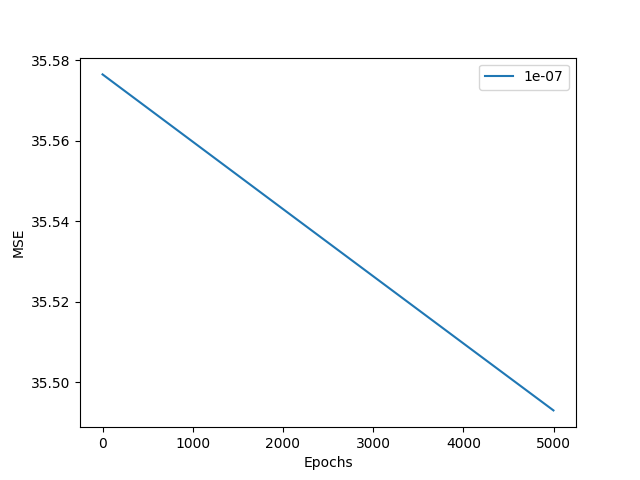
\includegraphics[width=0.32\textwidth, height=4cm]{1e-7} }}
    \subfloat[\centering Learning Rate = 1e-6]{{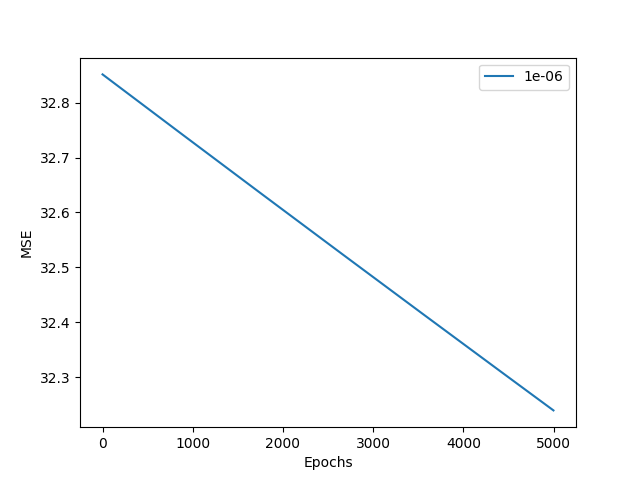
\includegraphics[width=0.32\textwidth, height=4cm]{1e-6} }}\\
    \subfloat[\centering Learning Rate = 1e-5]{{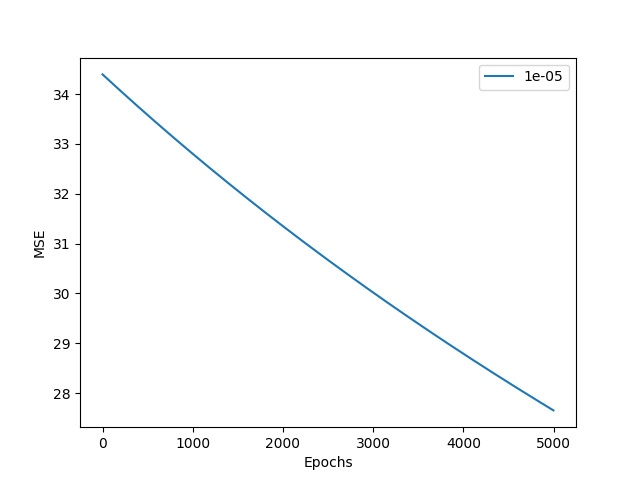
\includegraphics[width=0.32\textwidth, height=4cm]{1e-5} }}
    \subfloat[\centering Learning Rate = 1e-4]{{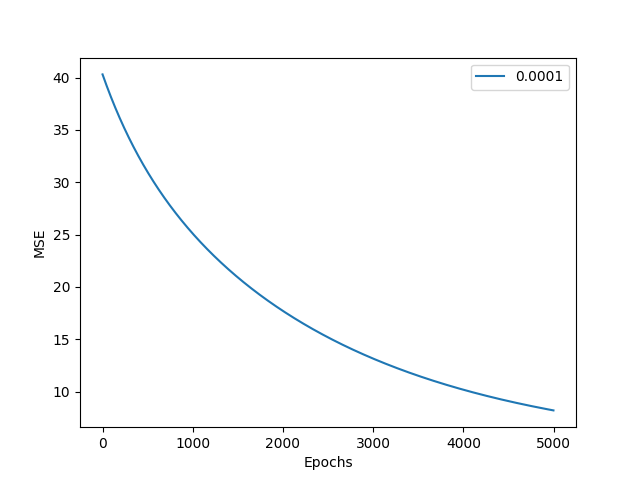
\includegraphics[width=0.32\textwidth, height=4cm]{1e-4} }}
    \subfloat[\centering Learning Rate = 1e-3]{{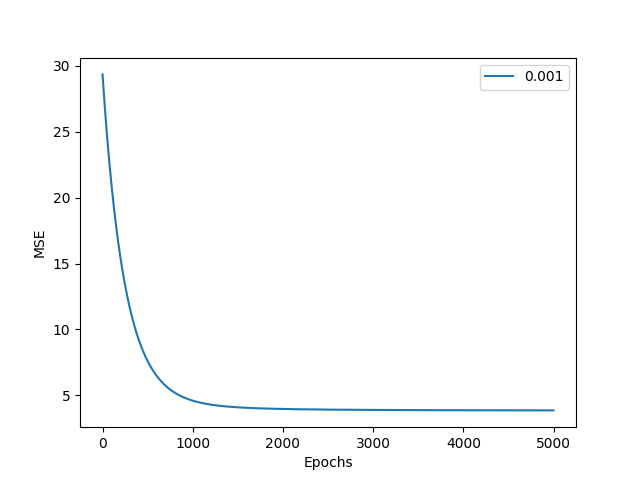
\includegraphics[width=0.32\textwidth, height=4cm]{1e-3} }}\\
    \subfloat[\centering Learning Rate = 1e-2]{{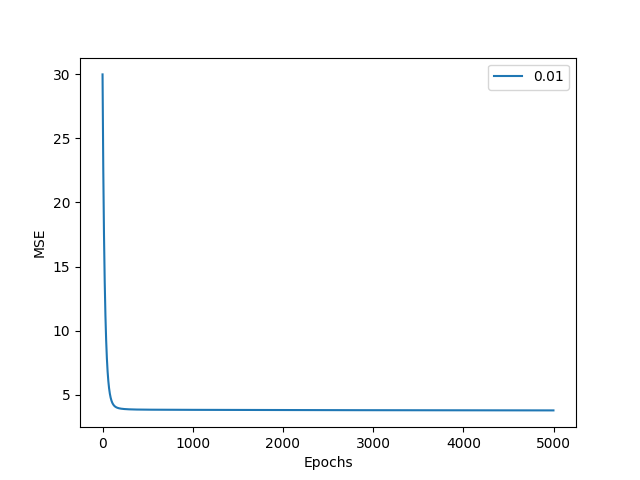
\includegraphics[width=0.32\textwidth, height=4cm]{1e-2} }}
    \subfloat[\centering Learning Rate = 1e-1]{{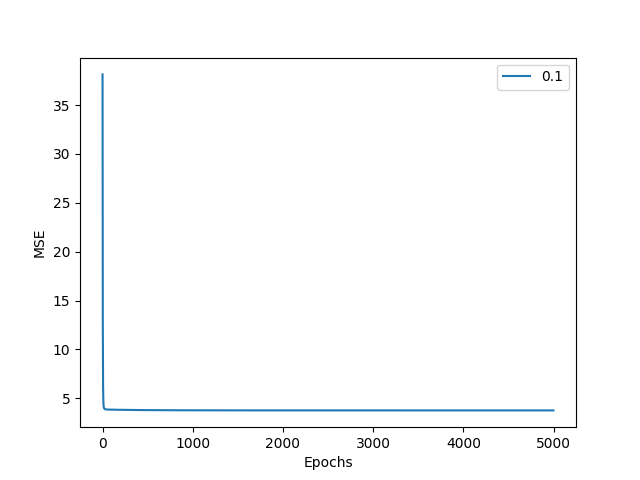
\includegraphics[width=0.32\textwidth, height=4cm]{1e-1} }}    
	 \subfloat[\centering Learning Rate = 1]
{{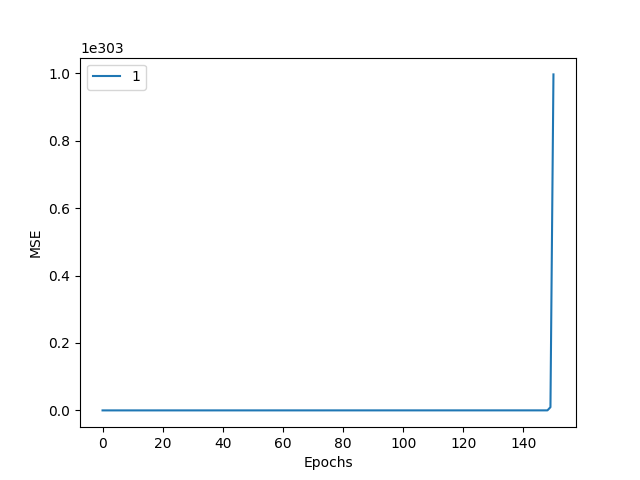
\includegraphics[width=0.32\textwidth, height=4cm]{1} }}\\
    \subfloat[\centering Learning Rate = 10]{{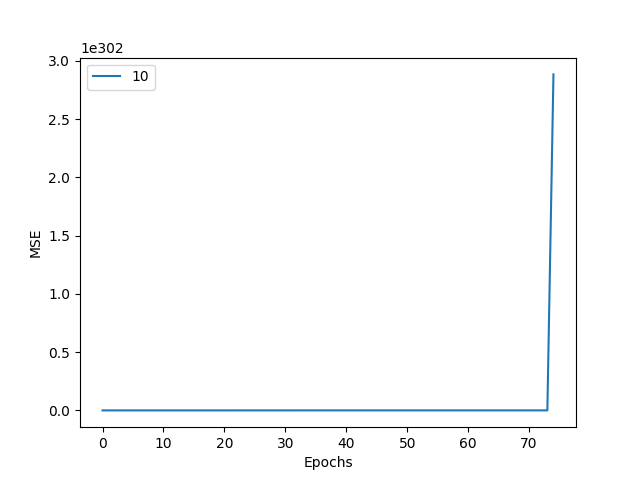
\includegraphics[width=0.32\textwidth, height=4cm]{10} }}\\
\caption{MSE vs Iterations for Normalized Data}
    \label{fig:normalized}%
\end{figure}


\textbf{Part 2.}a. None of the mentioned learning rates work for un-normalized data. With further reduction in learning rate, we see that a lr of $1e-11$ or $1e-12$ works well. As compared to the normalized data, we see that the learning rate needed for convergence in the un-normalized data is much smaller. The un-normalized data also gives a much larger value of the loss, which causes divergence. Thus as a result it is easier to train the normalized data.Fig. \ref{fig:un-normalized} shows the plots for MSE vs Iterations for different learning rates.\\

b. The weights and MSE are provided in \textbf{Part2.pdf}. We see that a learning rate of $1e-11$ works best. Features with large un-normalized values such as $sqft\_lot$ and $sqft\_living$ have smaller weights in the un-normalized training version than in the normalized version. Similarly, features with a smaller un-normalized value like the $month$ and $day$ have larger weights in the un-normalized training. We can attribute this to the impact of each feature on the price. When normalized, each feature contibutes equally to the price if the corresponding weights are equal. Therefore in the normalized situation, the weights highlight the impact of each feature on the price. However, in the un-normalized case, if all weights were one, larger features would impact the price more than smaller features. Thus, the weights in this case do not directly show the impace of each feature on the price, thus causing the experiments to be skewed.\\


\begin{figure}[h]
    \centering
    \subfloat[\centering Learning Rate = 1e-12]{{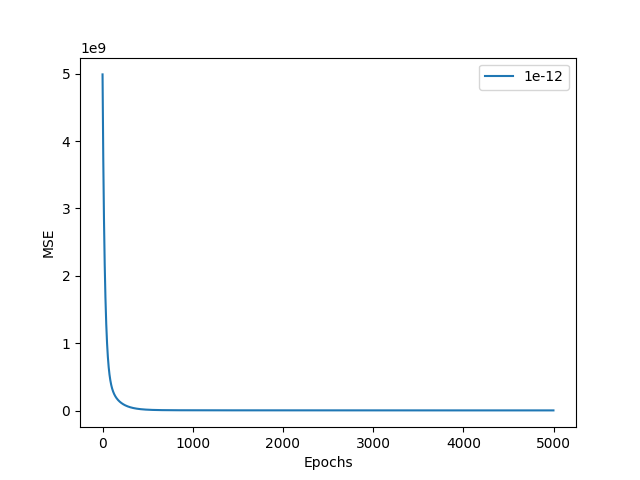
\includegraphics[width=0.32\textwidth, height=4cm]{1e-12_nn} }}
    \subfloat[\centering Learning Rate = 1e-11]{{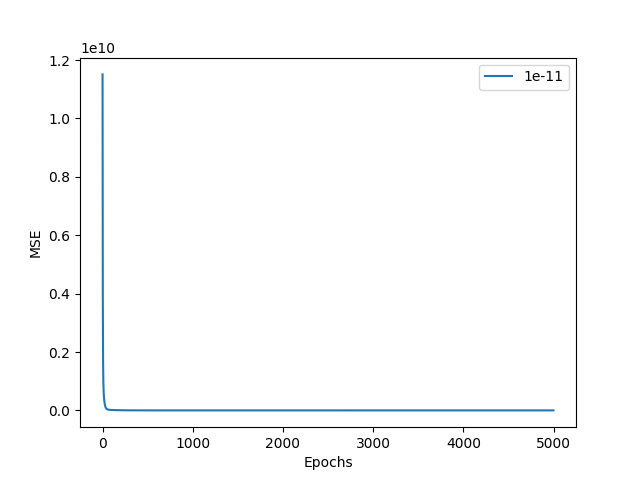
\includegraphics[width=0.32\textwidth, height=4cm]{1e-11_nn} }}
    \subfloat[\centering Learning Rate = 1e-8]{{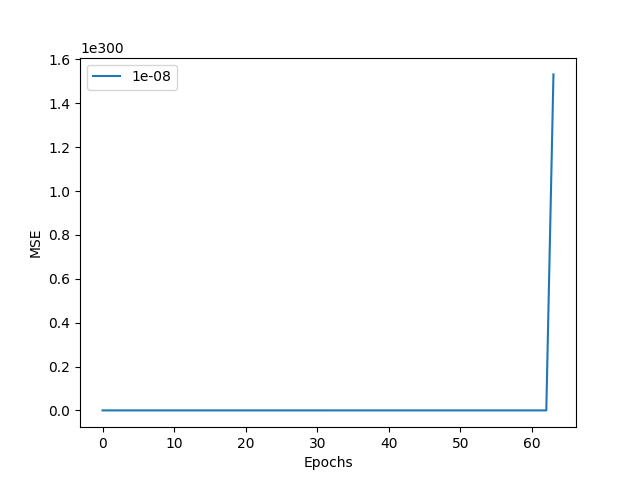
\includegraphics[width=0.32\textwidth, height=4cm]{1e-8_nn} }}\\
    \subfloat[\centering Learning Rate = 1e-7]{{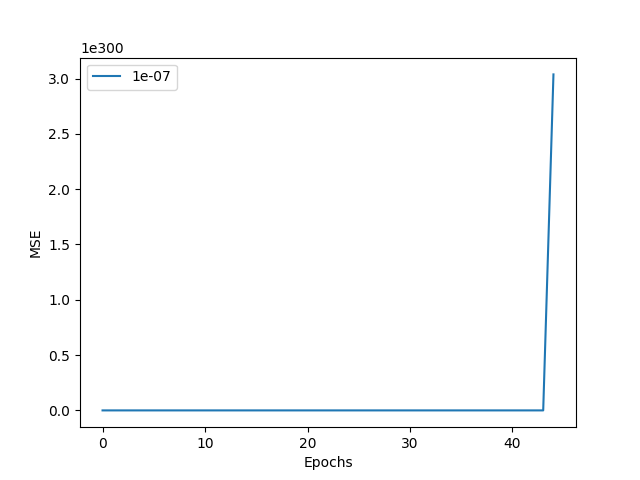
\includegraphics[width=0.32\textwidth, height=4cm]{1e-7_nn} }}
    \subfloat[\centering Learning Rate = 1e-6]{{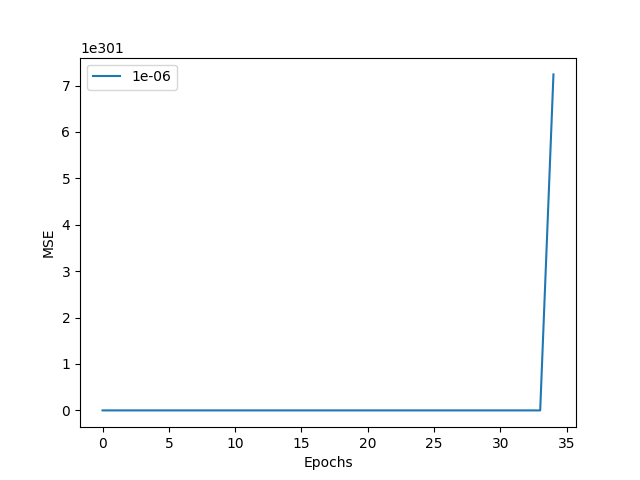
\includegraphics[width=0.32\textwidth, height=4cm]{1e-6_nn} }}
    \subfloat[\centering Learning Rate = 1e-5]{{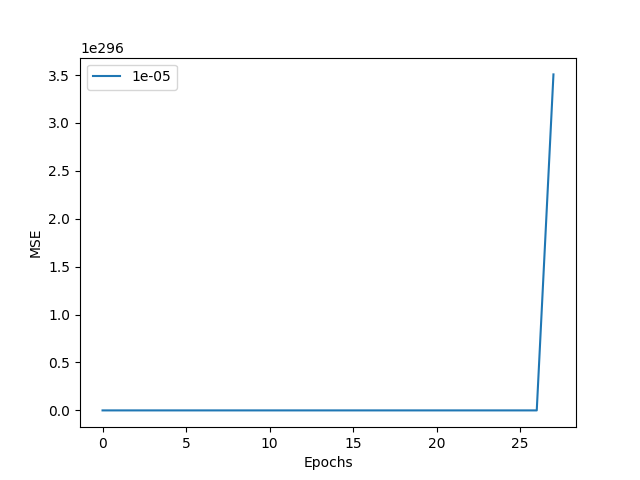
\includegraphics[width=0.32\textwidth, height=4cm]{1e-5_nn} }}\\
    \subfloat[\centering Learning Rate = 1e-4]{{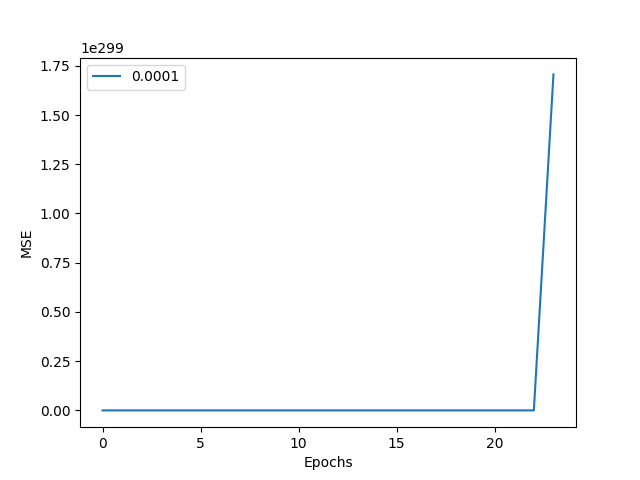
\includegraphics[width=0.32\textwidth, height=4cm]{1e-4_nn} }}
    \subfloat[\centering Learning Rate = 1e-3]{{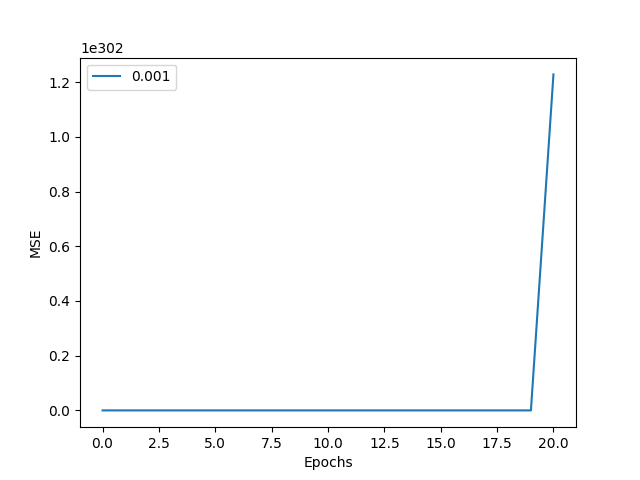
\includegraphics[width=0.32\textwidth, height=4cm]{1e-3_nn} }}
	\subfloat[\centering Learning Rate = 1e-2]{{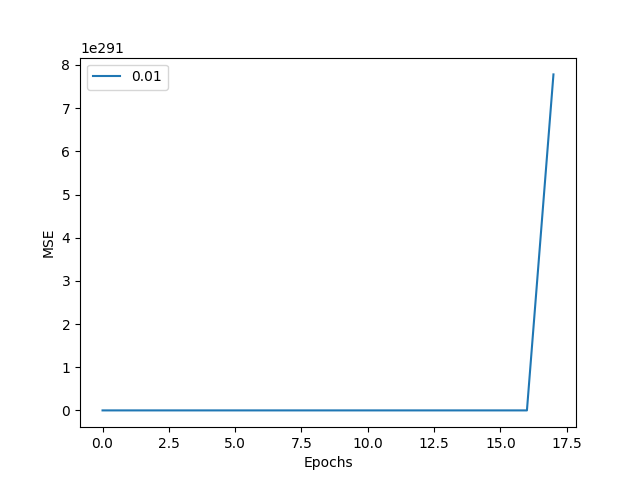
\includegraphics[width=0.32\textwidth, height=4cm]{1e-2_nn} }}\\
    \subfloat[\centering Learning Rate = 1e-1]{{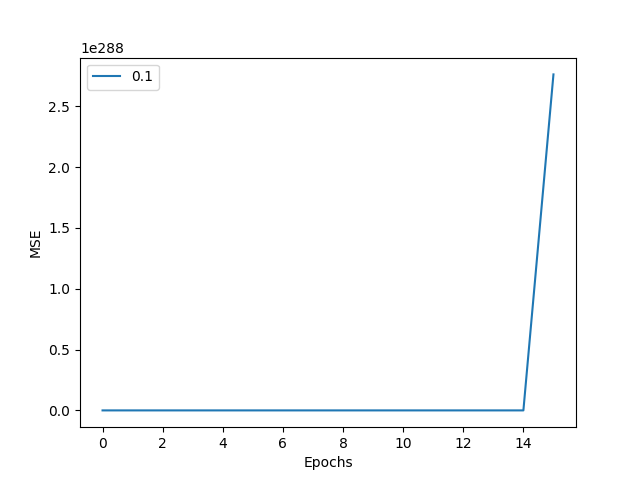
\includegraphics[width=0.32\textwidth, height=4cm]{1e-1_nn} }}    
	 \subfloat[\centering Learning Rate = 1]
{{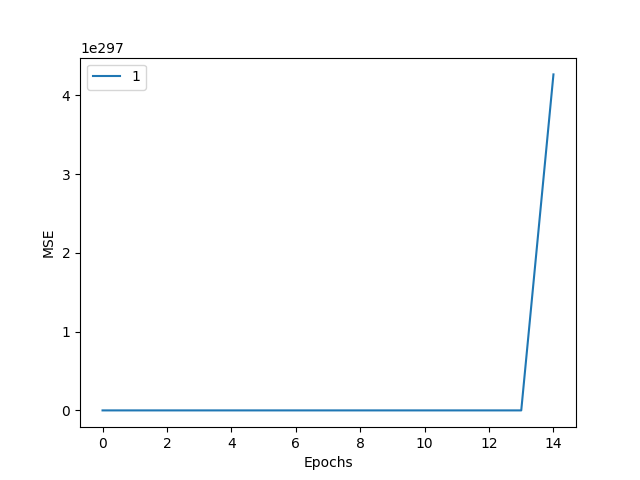
\includegraphics[width=0.32\textwidth, height=4cm]{1_nn} }}
    \subfloat[\centering Learning Rate = 10]{{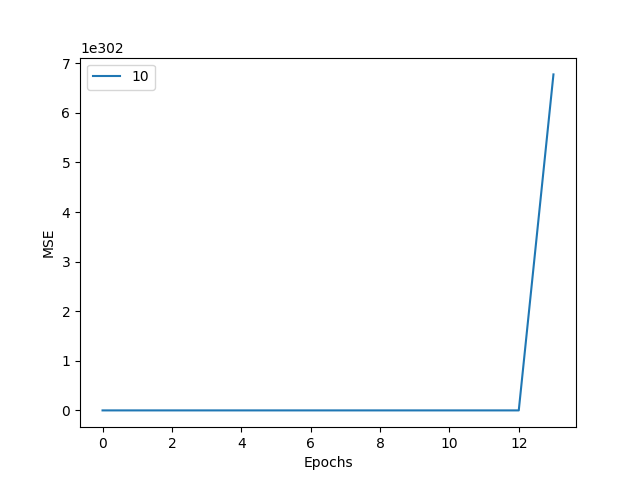
\includegraphics[width=0.32\textwidth, height=4cm]{10_nn} }}\\
\caption{MSE vs Iterations for Un-Normalized Data}
\label{fig:un-normalized}%
\end{figure}


\textbf{Part3.} The training MSE is $3.764$, and Validation MSE is $4.517$. Weights and results are provided in \textbf{Part3.pdf}. The new model has similar performance as the one used in Part 1. We see that the weights for $sqft\_living$ is larger in Part 3 ($0.3808$) than in Part 1. ($0.3638$). The weight for $sqft\_living$ in Part 3 is almost close to the sum of weights of $sqft\_living$ and $sqft\_living15$ from Part 1. It is slightly different because these two features aren't exactly the same. In general, for highly correlated features, I think the weights when just training $w_{1}$ would be almost the sum of the weights obtained from training $w_{1}$ and $w_{2}$. This is because if you consider the two features, the model is of the form $w_{1}x_{1} + w_{2}x_{2}$ in the first case, and $Wx_{1}$ in the second. If $x_{1} = x_{2}$, then we can see that after optimizing and reaching minimal error, $y = Wx_{1} = w_{1}x_{1} + w_{2}x_{2} \Rightarrow W = w_{1} + w_{2}$. \\ \\

\textbf{Part4.} In this section, I list out the methods which I tried, and those that worked

\begin{itemize}
\item Firstly, I tried defining date as an encoded format, with each combination of day, month and year having a unique encoded value. I use:
\begin{equation}
date_{encoded} = year + 100*month + day
\end{equation}
I thought that the selling price would be dependent on the date, month and year. However, the price was only dependent on the year, so this attempt didn't give increase in performance.
\item Next, the model seemed to overfit as the training loss was lower than the validation loss. So I tried removing a few features. To do this I recorded the weights of each feature, and removed the ones with the lowest weight. 
\item Then I tries to check the effect of half bathrooms on the price. This didn't result in much change either
\item Finally I tried synthesisng non-linear features, like the ration of $bedrooms$ to $bathrooms$, ratio of $sqft\_living$ to $sqft\_lot$, and so on. These seemed to be the most effective in improving the MSE.
\item One more thing I would have liked to tried with sufficient time and computing is to generate non-linear combinations of each data feature with the others, and observe which contributed the most to improving error.
\end{itemize}

\end{document}